\documentclass[14pt, a4paper]{article}
\usepackage{minitoc}
\usepackage[left=3.00cm, right=2.5cm, top=2.00cm, bottom=2.00cm]{geometry}
\usepackage{amsmath}
\usepackage{amssymb}
\usepackage{amsthm}
\usepackage{thmtools}
\usepackage{mathtools}
\usepackage{graphicx}
%\usepackage{algpseudocode}
%\usepackage{algorithm}
\usepackage[ruled,vlined,linesnumbered,algosection]{algorithm2e}
\usepackage{blindtext}
\usepackage{setspace}
\usepackage[utf8]{inputenc}
\usepackage[utf8]{vietnam}
\usepackage[center]{caption}
\usepackage[shortlabels]{enumitem}
\usepackage{fancyhdr} % header, footer
\usepackage{hyperref} % loại bỏ border với mục lục và công thức
\usepackage[nonumberlist, nopostdot, nogroupskip]{glossaries}
\usepackage{glossary-superragged}
\usepackage{tikz,tkz-tab}
\setglossarystyle{superraggedheaderborder}
\pagestyle{fancy}
%\usepackage[style=numeric,sortcites]{biblatex}
%\addbibresource{ref.bib}
%\usepackage[numbers]{natbib}
\usepackage{indentfirst}
\usepackage{multirow}
\usepackage[natbib,backend=biber,style=ieee, sorting=ynt]{biblatex}
\usepackage{cancel}
\bibliography{ref.bib}

\graphicspath{{./figures/}}


\hypersetup{
    colorlinks=false,
    pdfborder={0 0 0},
}


\fancyhf{}
\rhead{\textbf{Môn học: Các phương pháp ngẫu nhiên và ứng dụng}}
\lhead{\textbf{GVHD: PGS. TS. Tạ Công Sơn}}
\rfoot{\thepage}
\lfoot{\textbf{Học viên thực hiện: Nguyễn Chí Thanh - 21007925}}
\renewcommand{\headrulewidth}{0.4pt}
\renewcommand{\footrulewidth}{0.4pt}


\numberwithin{equation}{section}
\numberwithin{figure}{section}

\setlength{\parindent}{0.5cm}

\setcounter{secnumdepth}{3} % Cho phép subsubsection trong report
\setcounter{tocdepth}{3} % Chèn subsubsection vào bảng mục lục

\newtheorem{dl}{Định lý}
\newtheoremstyle{sltheorem}
{}                % Space above
{}                % Space below
{\normalfont}        % Theorem body font % (default is "\upshape")
{}                % Indent amount
{\bfseries}       % Theorem head font % (default is \mdseries)
{.}               % Punctuation after theorem head % default: no punctuation
{ }               % Space after theorem head
{}                % Theorem head spec
\theoremstyle{sltheorem}
\newtheorem{vd}{Ví dụ}
\newtheoremstyle{soltheorem}
{}                % Space above
{}                % Space below
{\normalfont}        % Theorem body font % (default is "\upshape")
{}                % Indent amount
{\bfseries}       % Theorem head font % (default is \mdseries)
{.}               % Punctuation after theorem head % default: no punctuation
{\newline}               % Space after theorem head
{}                % Theorem head spec
\theoremstyle{soltheorem}
\newtheorem*{loigiai}{Lời giải}

\numberwithin{dl}{section}
\numberwithin{vd}{section}

\doublespacing

\begin{document}
    \begin{titlepage}

        \newcommand{\HRule}{\rule{\linewidth}{0.5mm}} % Defines a new command for the horizontal lines, change thickness here

        \center % Center everything on the page

        %----------------------------------------------------------------------------------------
        %	HEADING SECTIONS
        %----------------------------------------------------------------------------------------
        \textsc{\LARGE Đại học Quốc Gia Hà Nội}\\[0.5cm]
        \textsc{\LARGE Trường đại học Khoa học tự nhiên}\\[0.5cm] % Name of your university/college
        \textsc{\LARGE Khoa Toán - Cơ - Tin học}\\[0.5cm]

        
\includegraphics[scale=0.2]{HUS-logo.jpg}\\[0.5cm]

        \textsc{\Large Chuyên ngành: Khoa học dữ liệu}\\[0.5cm] % Major heading such as course name


        %----------------------------------------------------------------------------------------
        %	TITLE SECTION
        %----------------------------------------------------------------------------------------

        \HRule \\[0.4cm]
        { \huge \bfseries TIỂU LUẬN MÔN HỌC}\\[0.4cm] % Title of your document
        \HRule \\[1.5cm]

        \textsc{\Large Môn học: Các phương pháp ngẫu nhiên và ứng dụng}\\[1cm] % Minor heading such as course title


        \textsc{\Large Đề tài: Xích Markov và Lý thuyết phân nhánh}\\[2cm]


        %----------------------------------------------------------------------------------------
        %	AUTHOR SECTION
        %----------------------------------------------------------------------------------------
        \begin{minipage}{0.4\textwidth}
            \begin{flushleft} \large
            \emph{Giảng viên hướng dẫn:} \\
            PGS. TS. Tạ Công Sơn % Supervisor's Name
            \end{flushleft}
        \end{minipage}\\[0.5cm]

        \begin{minipage}{0.4\textwidth}
        \begin{flushleft} \large
        \emph{Học viên thực hiện:}\\
        Nguyễn Chí Thanh \\
        MSHV: 21007925 \\ % Your name
        Lớp: Khoa học dữ liệu - K4
        \end{flushleft}
        \end{minipage}


        % If you don't want a supervisor, uncomment the two lines below and remove the section above
        %\Large \emph{Author:}\\
        %John \textsc{Smith}\\[3cm] % Your name

        %----------------------------------------------------------------------------------------
        %	DATE SECTION
        %----------------------------------------------------------------------------------------

        % I don't want day because it is English
        % {\large \today}\\[2cm] % Date, change the \today to a set date if you want to be precise

        %----------------------------------------------------------------------------------------
        %	LOGO SECTION
        %----------------------------------------------------------------------------------------

        %\includegraphics{logo/rsz_3logo-khtn.png}\\[1cm] % Include a department/university logo - this will require the graphicx package

        %----------------------------------------------------------------------------------------

        \vfill % Fill the rest of the page with whitespace

    \end{titlepage}

    \cleardoublepage
    \pagenumbering{gobble}
    \tableofcontents
    \newpage
    \listoffigures
    \newpage
    \glsaddall 
    \renewcommand*{\glossaryname}{Danh mục các từ viết tắt}
    \renewcommand*{\acronymname}{Danh sách từ viết tắt}
    \renewcommand*{\entryname}{Viết tắt}
    \renewcommand*{\descriptionname}{Viết đầy đủ}
    \printnoidxglossary
    \cleardoublepage
    \pagenumbering{arabic}

    %\maketitle

    \newpage

    \nocite{*}

    \begin{center}
    \section*{LỜI MỞ ĐẦU}
    \end{center}
    \addcontentsline{toc}{section}{{\bf LỜI MỞ ĐẦU}\rm}

    \newpage

    \section{Số bước trung bình chuyển tiếp giữa các trạng thái tạm thời}

    Ta xét một xích Markov trạng thái hữu hạn và giả định rằng các trạng thái được đánh số $T=\lbrace 1, 2, \dots, t \rbrace$ ký hiệu tập các trạng thái tạm thời.
    Ta đặt:

    \begin{equation*}
        \mathbf{P}_T = \begin{bmatrix} P_{11} & P_{12} & \dots & P_{1t} \\ \vdots & \vdots & \vdots & \vdots \\ P_{t1} & P_{t2} & \dots & P_{tt}  \end{bmatrix}
    \end{equation*}

    Và ta cần chú ý rằng ma trận $\mathbf{P}_T$ chỉ xác định xác suất chuyển tiếp từ các trạng thái tạm thời sang trạng thái tạm thời, và tổng của một số hàng nhỏ hơn 1 (mặt khác $T$ có thể là một tập đóng của các trạng thái).
    
    Ta xét hai trạng thái tạm thời $i$ và $j$, ta đặt $s_{ij}$ ký hiệu là số bước kỳ vọng mà xích Markov đến trạng thái $j$, khi ta biết xích Markov bắt đầu ở trạng thái $i$.
    Đặt $\delta_{i,j}=1$ khi $i=j$ và bằng 0 nếu ngược lại.
    Ta tính $s_{ij}$ sử dụng công thức kỳ vọng đầy đủ:

    \begin{equation} \label{eq:expected_number_periods_i_to_j}
        \begin{aligned}
            s_{ij} &= \delta_{i,j} + \sum_{k \in T} P_{ik}s_{kj} \\
            &= \delta_{i,j} + \sum_{k=1}^t P_{ik} s_{kj}
        \end{aligned}
    \end{equation}

    với đẳng thức cuối cùng của công thức trên cho ta thấy không thể chuyển từ một trạng thái hồi quy sang một trạng thái tạm thời, ý nghĩa rằng $s_{kj}=0$ khi $k$ là một trạng thái hồi quy.

    Ta đặt $\mathbf{S}$ ký hiệu là ma trận với các giá trị $s_{ij}, i, j = 1, \dots, t$. Ta có ma trận $\mathbf{S}$:

    \begin{equation*}
        \mathbf{S} = \begin{bmatrix} s_{11} & s_{12} & \dots & s_{1t} \\ \vdots & \vdots & \vdots & \vdots \\ s_{t1} & s_{t2} & \dots & s_{tt}  \end{bmatrix}
    \end{equation*}

    Ta viết lại công thức \ref{eq:expected_number_periods_i_to_j} dưới dạng ma trận:

    \begin{equation*}
        \mathbf{S} = \mathbf{I} + \mathbf{P}_T \mathbf{S}
    \end{equation*}

    với $\mathbf{I}$ là ma trận đơn vị kích thước $t$. Bởi vì công thức trên tương đương với:

    \begin{equation*}
        (\mathbf{I} - \mathbf{P}_T) \mathbf{S} = \mathbf{I}
    \end{equation*}

    Bằng cách nhân cả hai vế với $(\mathbf{I} - \mathbb{P}_T)^{-1}$ ta thu được:

    \begin{equation*}
        \mathbf{S} = (\mathbf{I} - \mathbf{P}_T)^{-1}
    \end{equation*}

    Với mỗi đại lượng $s_{ij}, i \in T, j \in T$, ta có thể tính đại lượng này bằng cách lấy phần tử tại hàng $i$ và cột $j$ của ma trận nghịch đảo của ma trận $\mathbf{I} - \mathbf{P}_T$ (sự tồn tại của ma trận nghịch đảo này dễ dàng chứn minh được).

    \begin{vd} \label{vd:gambler-ruin-problem}
        Ta xét bài toán người đánh bạc với $p=0.4$ và $N=7$. Bắt đầu với 3 đô la, xác định:
        \begin{enumerate}[label=(\alph*)]
            \item Số ván kỳ vọng để người chơi bài có 5 đô la.
            \item Số ván kỳ vọng để người chơi bài có 2 đô la.
        \end{enumerate}
    \end{vd}

    \begin{loigiai}
        Ma trận $\mathbf{P}_T$ xác định các giá trị $P_{ij}, i, j \in \lbrace 1, 2, 3, 4, 5, 6 \rbrace$ được xác định như sau:

        \begin{equation*}
            \mathbf{P}_T = \begin{bmatrix}
                0 & 0.4 & 0 & 0 & 0 & 0 \\
                0.6 & 0 & 0.4 & 0 & 0 & 0 \\
                0 & 0.6 & 0 & 0.4 & 0 & 0 \\
                0 & 0 & 0.6 & 0 & 0.4 & 0 \\
                0 & 0 & 0 & 0.6 & 0 & 0.4 \\
                0 & 0 & 0 & 0 & 0.6 & 0 \\
            \end{bmatrix}
        \end{equation*}

        Ta tính nghịch đảo ma trận $\mathbf{I} - \mathbf{P}_T$, ta thu được:

        \begin{equation*}
            \mathbf{S}=(\mathbf{I}-\mathbf{P}_T)^{-1}=
            \begin{bmatrix}
            1.6149 & 1.0248 & 0.6314 & 0.3691 & 0.1943 & 0.0777 \\
            1.5372 & 2.5619 & 1.5784 & 0.9228 & 0.4857 & 0.1943 \\
            1.4206 & 2.3677 & 2.9990 & 1.7533 & 0.9228 & 0.3691 \\
            1.2458 & 2.0763 & 2.6299 & 2.9990 & 1.5784 & 0.6314 \\
            0.9835 & 1.6391 & 2.0763 & 2.3677 & 2.5619 & 1.0248 \\
            0.5901 & 0.9835 & 1.2458 & 1.4206 & 1.5372 & 1.6149
            \end{bmatrix}
        \end{equation*}

        Vì vậy ta thu được $s_{3,5}=0.9228$ (ván) và $s_{3,2}=2.3677$ (ván).
    \end{loigiai}

    Với $i \in T, j \in T$, đại lượng $f_{ij}$ chính là xác suất để để xích Markov tạo ra một quỹ đạo chuyển tiếp đạt đến trạng thái $j$ khi biết xích Markov bắt đầu từ trạng thái $i$ dễ dàng được xác định từ $\mathbf{P}_T$.
    Để xác định mối liên hệ, ta bắt đầu từ biệc sử dụng công thức tính $s_{ij}$ dựa trên hệ đầy đủ là xích Markov đã từng đi qua trạng thái $j$ hay chưa.
    Sử dụng công thức kỳ vọng đầy đủ ta thu được:

    \begin{equation*}
        \begin{aligned}
            s_{ij} &= E \lbrack \text{ số bước để đến được } j \vert \text{ bắt đầu tại } i, \text{ đã từng đi qua } j \rbrack f_{ij} \\ & + E \lbrack \text{ số bước để đến được } j \vert \text{ bắt đầu tại } i, \text{ chưa từng đi qua } j \rbrack (1 - f_{ij}) \\
            &= (\delta_{i, j} + s_{{jj}}) f_{ij} + \delta_{ij}(1 - f_{ij}) \\
            &= \delta_{i,j} + f_{ij} s_{jj}
        \end{aligned}
    \end{equation*}

    với $s_{jj}$ là số bước kỳ vọng cần thêm vào khi trạng thái $j$ đã đạt và tiếp tục một lần nữa quay lại trạng thái $j$.
    Giải phương trình trên ta thu được:

    \begin{equation*}
        f_{ij} = \dfrac{s_{ij} - \delta_{i,j}}{s_{jj}}
    \end{equation*}

    \begin{vd}
        Trong ví dụ \ref{vd:gambler-ruin-problem}, xác suất là bao nhiêu để người chơi có lúc có 1 đô la?
    \end{vd}

    \begin{loigiai}
        Với $s_{31}=1.4206$ và $s_{11}=1.6149$, ta thu được:
        
        \begin{equation*}
            f_{31} = \dfrac{s_{31}}{s_{11}}=0.8797
        \end{equation*}

        Để kiểm tra lại, ta chú ý rằng $f_{31}$ chính là xác suất người đánh bạc bắt đầu với 3 đô la và có 1 đô la trước khi đạt được 7 đô la.
        Đây chính là xác suất để người đánh bạc mất 2 đô la trước khi có thêm 4 đô la cũng bằng xác suất người đánh bạc bắt đầu với 2 đô la và thu cuộc trước khi đạt được 6 đô la.
        Vì vậy:

        \begin{equation*}
            f_{31} = - \dfrac{1 - (0.6/0.4)^2}{1-(0.6/0.4)^6}=0.8797
        \end{equation*}
        và kết quả trùng khớp với cách làm đầu tiên.
    \end{loigiai}

    Giả sử ta đang quan tâm đến số bước kỳ vọng để xích Markov đi đến một tập các trạng thái $A$, không nhất thiết phải là các trạng thái lặp lại.
    Ta có thể giả định về tình huống trước bằng cách làm cho tất cả các trạng thái trong $A$ là trạng thái hấp thụ bằng cách đặt lại xác suất chuyển tiếp của các trạng thái trong tập $A$ thỏa mãn:
    \begin{equation*}
        P_{ii} = 1, i \in A
    \end{equation*}

    Việc này biến các trạng thái trong tập $A$ thành trạng thái hồi quy, và biến đổi bất kỳ trạng thái nào ngoài tập $A$ nhưng cuối cùng cũng chuyển tiếp vào một trạng thái trong tập $A$ thành một trạng thái tạm thái.
    Vì vậy, cách tiếp cận trước đây của ta có thể được sử dụng
    
    \section{Các quá trình phân nhánh}
    
    Trong phần này ta sẽ xem xét một lớp các xích Markov được gọi là các \textit{quá trình phân nhánh}.
    Lớp xích Markov này có ứng dụng rất rộng rãi trong y học, xã hội học và khoa học kỹ thuật.
    
    Ta xét một quần thể bao gồm các cá thể có thể tạo ra các thế hệ tiếp theo cùng loài.
    Ta giả định rằng từng cá thể đến cuối thời gian sống tạo ra $j$ con với xác suất $P_j, j \geq 0$ và độc lập với số con được sinh ra bởi cá thể khác.
    Ta giả sử $P_j < 1 \forall j \geq 0$.
    Số cá thể ban đầu được ký hiệu là $X_0$, được gọi là kích cỡ của thế hệ thứ 0.
    Tất cả con cháu của thế hệ thứ 0 tạo thành thế hệ đầu tiên và kích thước của quần thể tại thế hệ này ký hiệu là $X_1$.
    Tổng quát, ta đặt $X_n$ ký hiệu là kích cỡ của thế hệ thứ $n$.
    Vì vậy $\lbrace X_n \rbrace_{n=0,1,\dots}$ là một xích Markov có không gian trạng thái là tập hợp các số nguyên không âm.
    
    Ta cần chú ý rằng trạng thái 0 là một trạng hồi quy, vì rõ ràng $P_{00}=1$.
    Ngoài ra nếu $P_0 > 0$, tất cả các trạng thái khác là trạng thái tạm thời.
    Điều này xảy ra khi $P_{i0}=P_0^i$ có ý nghĩa quần thể ban đầu có $i$ cá thể và có xác suất ít nhất $P_0^i$ sẽ không còn thế hệ nào nữa mà quần thể bao gồm $i$ cá thể.
    Hơn nữa, vì bất kỳ tập hữu hạn các trạng thái tạm thời $\lbrace 1, 2, \dots, n \rbrace$ sẽ được xích Markov đi qua một số hữu hạn lần, dẫn đến một kết luận quan trọng là nếu $P_0 > 0$, số lượng quần thể sẽ về 0 hoặc tiến đến vô cùng.
    
    Ta đặt:
    \begin{equation*}
        \mu = \sum_{j=0}^{\infty} j P_j
    \end{equation*}
    
    ký hiệu số các con trung bình do một cá thể sinh ra và đặt:
    \begin{equation*}
        \sigma^2 = \sum_{j=0}^{\infty} (j - \mu)^2 P_j
    \end{equation*}
    là phương sai của số các con được tạo ra bởi một cá thể.
    
    Ta giả định rằng $X_0 = 1$, ban đầu chỉ có duy nhất 1 cá thể.
    Ta tính $E \lbrack X_n \rbrack$ và $\mathrm{Var} (X_n)$, ta có thể viết:
    \begin{equation*}
        X_n = \sum_{i=1}^{X_n - 1} Z_i
    \end{equation*}

    với $Z_i$ biểu diễn số con cháu ở cá thể thứ $i$ của thế hệ thứ $n-1$.
    Ta tính kỳ vọng của $X_n$ bằng cách lấy điều kiện trên $X_{n-1}$, ta thu được:

    \begin{equation*}
        \begin{aligned}
            E \lbrack X_n \rbrack &= E \lbrack E \lbrack X_n \vert X_{n-1} \rbrack \rbrack \\
            &= E \Bigg \lbrack E \Bigg \lbrack \sum_{i=1}^{X_n - 1} Z_i \vert X_{n-1} \Bigg \rbrack \Bigg \rbrack \\
            &= E \lbrack X_{n-1} \mu \rbrack \\
            &= \mu E \lbrack X_{n-1} \rbrack
        \end{aligned}
    \end{equation*}

    ta sử dụng $E \lbrack Z_i \rbrack = \mu$. Vì $E \lbrack X_0 \rbrack = 1$, công thức trên trở thành:

    \begin{equation*}
        \begin{aligned}
            E \lbrack X_1 \rbrack &= \mu \\
            E \lbrack X_2 \rbrack &= \mu E \lbrack X_1 \rbrack = \mu^2 \\
            & \vdots \\
            E \lbrack X_n \rbrack &= \mu E \lbrack X_{n-1} \rbrack = \mu^n
        \end{aligned}
    \end{equation*}

    Tương tự, $\mathrm{Var} (X_n)$ có thể được tính sử dụng công thức phương sai có điều kiện:

    \begin{equation*}
        \mathrm{Var} (X_n) = E \lbrack \mathrm{Var} (X_n \vert X_{n-1}) \rbrack + \mathrm{Var} (E \lbrack X_n \vert X_{n-1} \rbrack)
    \end{equation*}

    Khi ta đã biết $X_{n-1}$, $X_n$ là tổng của $X_{n-1}$ biến ngẫu nhiên độc lập có phân bố $\lbrace P_j, j \geq 0 \rbrace$.
    Vì vậy:

    \begin{equation*}
        E \lbrack X_n \vert X_{n-1} \rbrack = X_{n-1} \mu, \mathrm{Var} (X_n \vert X_{n-1}) = X_{n-1} \sigma^2
    \end{equation*}

    Công thức phương sai có điều kiện bây giờ trở thành:

    \begin{equation*}
        \begin{aligned}
            \mathrm{Var}(X_n) & =E[X_{n-1} \sigma^2]+\mathrm{Var}(X_{n-1} \mu) \\
            &=\sigma^2 \mu^{n-1}+\mu^2 \mathrm{Var}(X_{n-1}) \\
            &=\sigma^2 \mu^{n-1}+\mu^2(\sigma^2 \mu^{n-2}+\mu^2 \mathrm{Var}(X_{n-2})) \\
            &=\sigma^2(\mu^{n-1}+\mu^n)+\mu^4 \mathrm{Var}(X_{n-2}) \\
            &=\sigma^2(\mu^{n-1}+\mu^n)+\mu^4(\sigma^2 \mu^{n-3}+\mu^2 \mathrm{Var}(X_{n-3})) \\
            &=\sigma^2(\mu^{n-1}+\mu^n+\mu^{n+1})+\mu^6 \mathrm{Var}(X_{n-3}) \\
            &=\cdots \\
            &=\sigma^2(\mu^{n-1}+\mu^n+\cdots+\mu^{2 n-2})+\mu^{2 n} \mathrm{Var}(X_0) \\
            &=\sigma^2(\mu^{n-1}+\mu^n+\cdots+\mu^{2 n-2})
        \end{aligned}
    \end{equation*}

    Vì vậy,

    \begin{equation}
        \begin{aligned}
            \mathrm{Var} (X_n) = \begin{cases}
                \sigma^2 \mu^{n-1} \Big ( \dfrac{1 - \mu^n}{1 - \mu} \Big) &\text{ nếu } \mu \neq 1 \\
                n \sigma^2 &\text{ nếu } \mu = 1
            \end{cases}
        \end{aligned}
    \end{equation}

    Ta đặt $\pi_0$ ký hiệu quần thể cuối cùng sẽ biến mất (với giả định là $X_0=1$). Về mặt hình thức:

    \begin{equation*}
        \pi_0 = \lim_{n \rightarrow \infty} P \lbrace X_n = 0 \vert X_0 = 1 \rbrace
    \end{equation*}

    Bài toán xác định giá trị $pi_0$ lần đầu tiên được đặt ra bởi Galton vào năm 1889 liên quan tới sự biến mất của một dòng họ.

    Ta thấy rằng $pi_0 = 1$ nếu $\mu < 1$ vì:

    \begin{equation*}
        \begin{aligned}
            \mu^n = E \lbrack X_n \rbrack &= \sum_{j=1}^{\infty} j P \lbrace X_n = j \rbrace \\
            & \geq \sum_{j=1}^{\infty} 1. P \lbrace X_n = j \rbrace \\
            & = P \lbrace X_n \geq 1 \rbrace
        \end{aligned}
    \end{equation*}

    Ta nhận thấy $\mu^n \rightarrow 0$ khi $\mu < 1$ kéo theo $P \lbrace X \geq 1 \rbrace \rightarrow 0$ vì vậy $P \lbrace X_n = 0 \rbrace \rightarrow 1$.

    Thực tế, ta có thể chỉ ra $\pi_0 = 1$ ngay cả khi $\mu = 1$.K
    Khi $\mu > 1$, ta thấy $\pi_0 < 1$, và công thức xác định $p_0$ nhận được bằng cách lấy điều kiện trên số con cháu của từng cá thể trong quần thể tại thế hệ 0:

    \begin{equation*}
        \begin{aligned}
            \pi_0 &= P \lbrace \text{quần thể biến mất} \rbrace \\
            &= \sum_{j=0}^{\infty} P \lbrace \text{quần thể biến mất} \vert X_1 = j \rbrace P_j
        \end{aligned}        
    \end{equation*}

    Bây giờ, khi biết $X_1 = j$, quần thể sẽ bị biến mất khi và chỉ khi nếu từng dòng họ trong $j$ dòng họ được bắt đầu bằng các cá thể của thế hệ thứ nhất biến mất.
    Ta giả sử từng dòng họ hoạt động độc lặp vì vậy, xác suất để từng dòng họ bị biến mất là $\pi_0$, ta thu được:
    
    \begin{equation*}
        P \lbrace \text{quần thể biến mất}\vert X_1 = j \rbrace = \pi_0^j
    \end{equation*}

    và $\pi_0$ thỏa mãn:

    \begin{equation} \label{eq:pi_0}
        \pi_0 = \sum_{j=0}^{\infty} \pi_0^j P_j
    \end{equation}

    Thực tế khi $\mu > 1$, ta có thể thấy $\pi_0$ là số dương nhỏ nhất thỏa mãn công thức \ref{eq:pi_0}.

    \begin{vd}
        Nếu $P_0 = \dfrac{1}{2}, P_1 = \dfrac{1}{4}, P_2 = \dfrac{1}{4}$. Xác định $\pi_0$
    \end{vd}

    \begin{loigiai}
        Vì $\mu = \dfrac{3}{4} \leq 1$ nên $\pi_0 = 1$
    \end{loigiai}

    \begin{vd} \label{vd:4.32}
        Nếu $P_0 = \dfrac{1}{4}, P_1 = \dfrac{1}{4}, P_2 = \dfrac{1}{2}$. Xác định $\pi_0$.
    \end{vd}

    \begin{loigiai} \label{vd:4.33}
        $\pi_0$ thỏa mãn:
        \begin{equation*}
            \pi_0 = \dfrac{1}{4} + \dfrac{1}{4} \pi_0 + \dfrac{1}{2} \pi_0^2
        \end{equation*}

        hoặc

        \begin{equation*}
            2 \pi_0^2 - 3 \pi_0 + 1 = 0
        \end{equation*}

        Nghiệm dương nhỏ nhất của phương trình bậc 2 này là $\pi_0 = \dfrac{1}{2}$
    \end{loigiai}

    \begin{vd}
        Trong ví dụ \ref{vd:4.32} và ví dụ \ref{vd:4.33}, xác suất cả quần thì bị biến mất là bao nhiêu nếu ban đầu bao gồm $n$ cá thể?
    \end{vd}

    \begin{loigiai}
        Khi cả quần thể bị biến mất khi và chỉ khi tất cả các dòng họ của từng thành viên của thế hệ ban đầu biến mất, xác suất này là $\pi_0^n$.
        Ví dụ \ref{vd:4.32} thu được $\pi_0^n = 1$, và cho ví dụ \ref{vd:4.33}, $\pi_0^n = \Big ( \dfrac{1}{2} \Big )^n$
    \end{loigiai}

    \section{Xích Markov đảo ngược thời gian}

    Ta xét một xích Markov ergodic dừng (là một xích Markov đã được vận hành một thời gian dài) có xác suất chuyển trạng thái $P_{ij}$ và phân bố dừng $\pi_i$ và ta giả sử rằng tại một vài thời điểm ta lưu vết dãy các trạng thái đi ngược thời gian.
    Bắt đầu ở thời điểm, ta xét dãy các trạng thái $X_n, X_{n-1}, X_{n-2}, \dots$.
    Ta nhận thấy dãy trạng thái này cũng là một xích Markov với xác suất chuyển trạng thái $Q_{ij}$ được định nghĩa bởi:

    \begin{equation*}
        \begin{aligned}
            Q_{ij} &= P \lbrace X_m = j \vert X_{m+1} = i \rbrace \\
            &= \dfrac{P \lbrace X_m = j, X_{m+1}=i \rbrace}{P \lbrace X_{m+1}=i \rbrace} \\
            &= \dfrac{P \lbrace X_m = j \vert X_{m+1} = i \rbrace P \lbrace X_{m+1=i \vert X_m = j \rbrace}}{P \lbrace X_{m+1}=j \rbrace} \\
            &= \dfrac{\pi_j P_{ji}}{\pi_i}
        \end{aligned}
    \end{equation*}

    Để chứng minh quá trình ngược thực sự là một xích Markov ta cần kiểm chứng:

    \begin{equation*}
        P \lbrace X_m = j \vert X_{m+1}=i, X_{m+2}, X_{m+3}, \dots \rbrace P \lbrace X_m = j \vert X_{m+1}=i \rbrace
    \end{equation*}

    Ta xét thời điểm hiện tại là $m+1$. Khi $X_0, X_1, X_2, \dots$ là một xích Markov, phân bố có điều kiện của các trạng thái tương lai $X_{m+2}, X_{m+3}, \dots$ khi cho trạng thái hiện tại $X_{m+1}$ độc lập vào trạng thái quá khứ $X_m$.
    Tuy nhiên, tính độc lập là một mối quan hệ đối xứng (nếu A độc lập với B thì B cũng độc lập với A) và vì vậy khi biết $X_{m+1}$ thì $X_m$ độc lập với $X_{m+2}, X_{m+3}, \dots$ và đây chính xác là việc ta cần kiểm chứng.

    Vì vậy, quá trình ngược cũng là một xích Markov với xác suất chuyển trạng thái được tính bởi công thức:

    \begin{equation*}
        Q_{ij} = \dfrac{\pi_j P_{ji}}{\pi_i}
    \end{equation*}

    Nếu $Q_{ij} = P_{ij}$ với mọi $i, j$ khi đó xích Markov được gọi là khả đảo thời gian.
    Điều kiện cho việc khả đảo thời gian $Q_{ij}=P_{ij}$ có thể được biểu diễn bởi:

    \begin{equation} \label{eq:Time-Reversible}
        \pi_i P_{ij} = \pi_j P_{ji} \forall i, j
    \end{equation}

    Điều kiện trong công thức \ref{eq:Time-Reversible} có thể được phát biểu là với mọi trạng thái $i$ và $j$, tỷ lệ quá trình đi từ $i$ đến $j$ ($\pi_i P_{ij}$) bằng với tỷ lệ quá trình đi từ $j$ đến $i$ ($\pi_j P_{ji}$).
    Một điều rất cần chú ý là điều kiện cần hiển nhiên cho tính khả đảo thời gian là chuyển tiếp từ $i$ đến $j$ khi đi ngược thời gian tương đương với chuyển tiếp từ $j$ sang $i$ khi đi theo thuận chiều thời gian.
    Nếu $Xm=i$ và $X_{m-1}=j$ thì một phép biến đổi từ $i$ sang $j$ được quan sát nếu ta quan sát ngược thời gian và một từ $j$ sang $i$ nếu ta nhìn thuận chiều thời gian.
    Vì vậy, tỷ lệ mà quá trình thuận tạo ra một chuyên tiếp từ $j$ sang $i$ luôn luôn bằng với tỷ lệ quá trình ngược tạo ra một chuyển tiếp từ $i$ sang $j$.
    Nếu khả đảo thời gian, tỷ lệ tạo ra một chuyển trạng thái từ $i$ sang $j$ của quá trình thuận và quá trình ngược phải bằng nhau.

    Nếu ta có thể tìm các số không âm, tổng bằng 1 và thỏa mãn phương trình \ref{eq:Time-Reversible}, khi đó xích Markov là khả đảo thời gian và các số biểu diễn phân bố tới hạn. Nếu:

    \begin{equation}
        x_i P_{ij} = x_j P_{ji} \thickspace \forall i, j \thickspace \sum_{i} x_i = 1
    \end{equation}

    sau đó cổng tổng theo $i$ ta thu được:

    \begin{equation*}
        \sum_i x_i P_{ij} = x_j \sum_i P_{ji} = x_j, \thickspace \sum_{i} x_i = 1
    \end{equation*}

    và phân bố tới hạn $\pi_i$ chính là nghiệm duy nhất của phương trình trên nên $x_i = \pi_i$ với mọi $i$.

    \begin{vd} \label{vd:4.35}
        Ta xét các bước đi ngẫu nhiên với trạng thái $0, 1, \dots, M$ và xác suất chuyển trạng thái:

        \begin{equation*}
            \begin{cases}
                P_{i, i+1} = \alpha_i = 1 - P_{i, i - 1}, \thickspace i=1, \dots, M-1 \\
                P_{0, 1} = \alpha_0 = 1 - P_{0, 0} \\
                P_{M,M} = \alpha_M - P_{M, M-1}
            \end{cases}
        \end{equation*}
    \end{vd}

    \begin{loigiai}
        Không cần tính toán, ta có thể khẳng định đây là một xích Markov, quá trình này chỉ có thể tạo ra các chuyển tiếp từ một trạng thái sang hai trạng thái gần nhất, vì vậy xích Markov khả đảo theo thời gian.
        Điều này xảy ra khi ta chú ý rằng số chuyển trạng thái từ $i$ sang $i+1$ tất cả phải nằm trong 1 trong các số từ $i+1$ sang $i$.
        Bởi vì giữa hai chuyển tiếp bất kỳ từ $i$ sang $i+1$ phải có một lần chuyển từ $i+1$ sang $i$ (và ngược lại) vì vậy chỉ có duy nhất để quay lại trạng thái $i$ từ một trạng thái cao hơn bằng cách đi qua trạng thái $i+1$.
        Vì vậy, tỷ lệ chuyển tiếp từ $i$ sang $i+1$ bằng tỷ lệ từ $i+1$ sang $i$ và vì vậy quá trình là khả đảo thời gian.

        Ta có thể dễ dàng tìm phân bố giới hạn bằng cách với mỗi trạng thái $i=0,1,\dots,M-1$, xác suất mà quá trình chuyển từ trạng thái $i$ sang trạng thái $i+1$ bằng xác suất chuyển từ trạng thái $i+1$ sang trạng thái $i$.
        Ta thu được:
        
        \begin{equation*}
            \begin{aligned}
                \pi_0 \alpha_0 &= \pi_1 (1 - \alpha_1) \\
                \pi_1 \alpha_1 &= \pi_2 (1 - \alpha_2) \\
                & \vdots \\
                \pi_i \alpha_i &= \pi_{i+1} (1 - \alpha_{i+1})
            \end{aligned}
        \end{equation*}

        Giải hệ phương trình trên theo $\pi_0$, ta thu dược:

        \begin{equation*}
            \begin{aligned}
                \pi_1 &= \dfrac{\alpha_0}{1-\alpha_1} \pi_0 \\
                \pi_2 &= \dfrac{\alpha_1}{1-\alpha_2} \pi_1 = \dfrac{\alpha_1 \alpha_0}{(1-\alpha_2)(1-\alpha_1)} \pi_0
            \end{aligned}
        \end{equation*}

        và tổng quát:

        \begin{equation*}
            \pi_i = \dfrac{\alpha_{i-1}\dots \alpha_0}{(1-\alpha_i)\dots(1-\alpha_1)} \pi_0, i = 1, 2, \dots, M
        \end{equation*}

        Vì $\sum_{0}^M \pi_i = 1$, ta thu được:

        \begin{equation*}
            \pi_0 \Bigg \lbrack 1 + \sum_{j=1}^M \dfrac{\alpha_{i-1}\dots \alpha_0}{(1-\alpha_i)\dots(1-\alpha_1)}  \Bigg \rbrack = 1
        \end{equation*}

        hoặc:

        \begin{equation} \label{eq:4.23}
            \pi_0 = \Bigg \lbrack 1 + \sum_{j=1}^M \dfrac{\alpha_{i-1}\dots \alpha_0}{(1-\alpha_i)\dots(1-\alpha_1)}  \Bigg \rbrack^{-1}
        \end{equation}

        và:

        \begin{equation} \label{eq:4.24}
            \pi_i = \dfrac{\alpha_{i-1}\dots \alpha_0}{(1-\alpha_i)\dots(1-\alpha_1)} \pi_0, i = 1, 2, \dots, M
        \end{equation}

        Ví dụ, nếu $\alpha_i \equiv \alpha $ khi đó:

        \begin{equation*}
            \begin{aligned}
                \pi_0 &= \Bigg \lbrack 1 + \sum_{j=1}^M \Big ( \dfrac{\alpha}{1-\alpha} \Big)^j \Bigg \rbrack^{-1} \\
                &= \dfrac{1-\beta}{1-\beta_{M+1}}
            \end{aligned}
        \end{equation*}

        và tổng quát:

        \begin{equation*}
            \pi_i = \dfrac{\beta_i (1 - \beta)}{1 - \beta_{M+1}}, i = 0, 1 , \dots, M
        \end{equation*}

        với:

        \begin{equation*}
            \beta = \dfrac{\alpha}{1 - \alpha}
        \end{equation*}
    \end{loigiai}

    Một trường hợp đặc biệt khác của ví dụ \ref{vd:4.35} là mô hình chiếc bình được nhà vật lý học T. Ehrenfest đề xuất để mô tả chuyển động của các phần tử.
    Ta giả sử rằng M phân tử được phân phối giữa hai bình và tại mỗi thời điểm một phân tử được chọn ngẫu nhiên, được lấy ra khỏi bình hiện tại và chuyển sang bình còn lại.
    Số phân tử trong bình là trường hợp đặc biệt của xích Markov trong ví dụ \ref{vd:4.35}:

    \begin{equation*}
        \alpha_i = \dfrac{M - i}{M}, i = 0, 1, \dots, M
    \end{equation*}

    Vì vậy, sử dụng công thức \ref{eq:4.23} và \ref{eq:4.24} phân bố giới hạn trong trường hợp này là:

    \begin{equation*}
        \begin{aligned}
            \pi_0 &= \Bigg \lbrack 1 + \sum_{j=1}^M \dfrac{(M-j+1) \dots (M-1)M}{j (j-1) \dots 1} \Bigg \rbrack^{-1} \\
            &= \Bigg \lbrack \sum_{j=0}^M \binom Mj \Bigg \rbrack^{-1} \\
            &= \Bigg ( \dfrac{1}{2} \Bigg )^M
        \end{aligned}
    \end{equation*}

    Ta sử dụng đồng nhất thức:

    \begin{equation*}
        \begin{aligned}
            1 &= \Big ( \dfrac{1}{2} + \dfrac{1}{2} \Big)^M \\
            &= \sum_{j=0}^M \binom{M}{j} \Bigg ( \dfrac{1}{2} \Bigg )^M
        \end{aligned}
    \end{equation*}

    Vì vậy, từ công thức \ref{eq:4.24}:

    \begin{equation*}
        \pi_i = \binom{M}{i} \Bigg ( \dfrac{1}{2} \Bigg)^M, i = 0, 1, \dots, M
    \end{equation*}

    Bởi vì công thức trên chỉ là phân bố nhị thức, vì vậy trong dài hạn, vị trí của từng quả cầu trong $M$ quả cầu độc lập và từng quả có thể ở hai bình với xác suất như nhau.
    Tuy nhiên, một cách khá trực quan, nếu ta chú ý vào một quả cầu bất kỳ, rất rõ ràng nếu vị trí của quả cầu độc lập so với vị trí của các quả cầu khác (vì không quan trọng $M-1$ quả cầu còn lại ở đâu, quả cầu khi được chú ý tại từng bước sẽ được di chuyển với xác suất $1/M$) và vì tính đối xứng, khả năng nó nằm trong một trong hai bình là như nhau.

    \begin{figure}[h!]
        \centering
        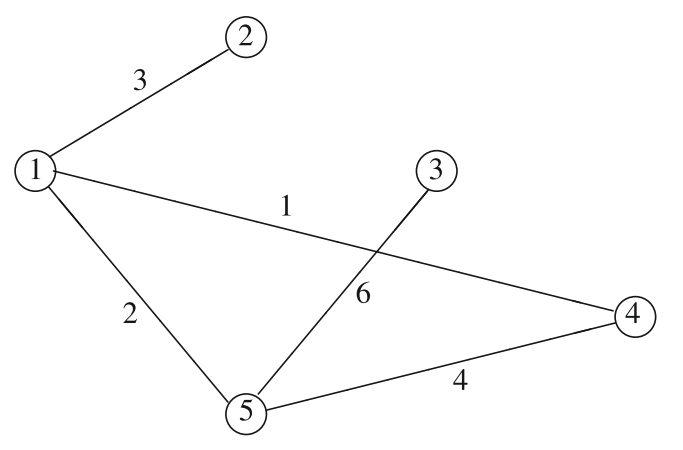
\includegraphics[scale=0.5]{1.png}
        \caption{Một đồ thị liên thông với trọng số của các cung}
        \label{fig:4.1}
    \end{figure}
\end{document}